%%%%%%%%%%%%%%%%%%%%%%%%%%%%%%%%%%%%%%%%%
% University/School Laboratory Report
% LaTeX Template
% Version 3.1 (25/3/14)
%
% This template has been downloaded from:
% http://www.LaTeXTemplates.com
%
% Original author:
% Linux and Unix Users Group at Virginia Tech Wiki 
% (https://vtluug.org/wiki/Example_LaTeX_chem_lab_report)
%
% License:
% CC BY-NC-SA 3.0 (http://creativecommons.org/licenses/by-nc-sa/3.0/)
%
%%%%%%%%%%%%%%%%%%%%%%%%%%%%%%%%%%%%%%%%%

%----------------------------------------------------------------------------------------
%	PACKAGES AND DOCUMENT CONFIGURATIONS
%----------------------------------------------------------------------------------------

\documentclass[12pt]{article}
\usepackage[left=3cm, right=3cm]{geometry}
\usepackage{natbib} % Required to change bibliography style to APA
\usepackage{amsmath} % Required for some math elements 
\usepackage{tabularx,booktabs,tabulary,array,graphicx,url}
\usepackage{graphicx}
\usepackage{multirow}
\usepackage{caption}
\usepackage{indentfirst}
%\usepackage{subcaption}
\usepackage{subfig}
\newcommand*\rot{\rotatebox{90}}


\renewcommand{\labelenumi}{\alph{enumi}.} % Make numbering in the enumerate environment by letter rather than number (e.g. section 6)

%\usepackage{times} % Uncomment to use the Times New Roman font

%----------------------------------------------------------------------------------------
%	DOCUMENT INFORMATION
%----------------------------------------------------------------------------------------

\title{Correction of keyboard typos with an Hidden Markov Model} % Title

\author{Ilaria Pigazzini, Cezar Angelo Sas, Andrea Vidali} %
% Author name

\date{\today} % Date for the report

\begin{document}

\maketitle % Insert the title, author and date

% \begin{center}
% \begin{tabular}{l r}
% Date Performed: & January 1, 2012 \\ % Date the experiment was performed
% Partners: & James Smith \\ % Partner names
% & Mary Smith \\
% Instructor: & Professor Smith % Instructor/supervisor
% \end{tabular}
% \end{center}

% If you wish to include an abstract, uncomment the lines below
% \begin{abstract}
% Abstract text
% \end{abstract}

%----------------------------------------------------------------------------------------
%	SECTION 1
%----------------------------------------------------------------------------------------
\newpage
\tableofcontents \newpage
\section{Introduction}
HMMispelling is a demo application to correct input keyboard typos. During the
development of our project we made some studies on the problem: we defined an
Hidden Markov Model, ran the Viterbi algorithm on it and analyzed the
results by comparing different configurations and inputs.
% To determine the atomic weight of magnesium via its reaction with oxygen and to study the stoichiometry of the reaction (as defined in \ref{definitions}):
% 
% \begin{center}\ce{2 Mg + O2 -> 2 MgO}\end{center}

% If you have more than one objective, uncomment the below:
%\begin{description}
%\item[First Objective] \hfill \\
%Objective 1 text
%\item[Second Objective] \hfill \\
%Objective 2 text
%\end{description}

\section{The model}
We modeled the problem as an hidden markov model, where the hidden states are
the characters of the text which should have been typed; the emissions are the
actual typed characters.

The chosen task to infer the correct typed text is �Most Likely Sequence�. The
Hidden Markov Model library(see Section~\ref{libraries}, Hidden-Markov Model) used in our
project implements the Viterbi algorithm.
% \label{definitions}
% \begin{description}
% \item[Stoichiometry]
% The relationship between the relative quantities of substances taking part in a reaction or forming a compound, typically a ratio of whole integers.
% \item[Atomic mass]
% The mass of an atom of a chemical element expressed in atomic mass units. It is approximately equivalent to the number of protons and neutrons in the atom (the mass number) or to the average number allowing for the relative abundances of different isotopes. 
% \end{description} 
 
%----------------------------------------------------------------------------------------
%	SECTION 2
%----------------------------------------------------------------------------------------
\subsection{Model Parameters}
% Table generated by Excel2LaTeX from sheet 'Foglio4'
Following, the parameters given to the model:
\begin{itemize}
	\item[]\emph{States}: alphabetical characters of the $QWERTY$ keyboard
	\item[]\emph{Emissions}: alphabetical characters of the $QWERTY$ keyboard
	\item[]\emph{Prior Probability Matrix}: relative frequencies of letters in the
	Englis language.
	\item[]\emph{Transition Matrix}: bigram frequencies of the English language. 
	See Section~\ref{transitionM} for further information.
	\item[]\emph{Emission Matrix}: the probability of the digit to be correct or
	uncorrect. The uncorrect digits for every QWERTY alphabetical character are its
	neighbors with distance one. See Section~\ref{emissionM} for further
	information.
\end{itemize}
Since the correction of mispelling will be applied on the alphabetical
characters(lowercase and uppercase, plus whitespace) of the $QWERTY$ keyboard,
in the following sections we will refer to keyboard input as ``digit''.
\subsection{Prior probability matrix}
To obtain this matrix we computed for every digit the frequency of the bigram
[whitespace, digit]. This matrix and the transition matrix were trained on the
same datasets~(see Section~\ref{dataset}).
\subsection{Transition matrix}\label{transitionM}

%how we obtained it
The transition matrix describes the probability of a digit to be followed by
another digit in the input text. The values of this matrix are bigram
frequencies of the English language, where a bigram is a sequence of two digits.
We trained this matrix on three datasets: \emph{Swift}, \emph{Twitter} and the
sum of the two, named \emph{Hybrid}(see Section~\ref{dataset}).
\subsection{Emission matrix}\label{emissionM}
%list the 3 different types
Consider a digit of the keyboard. In our model we assume that its neighbors are
all digit placed at distance ``$1$ digit'' in every direction on the keyboard.
For instance, digit ``$S$'' is at distance $1$ from digit ``$A$'' but it is at distance ``$2$'' from
digit ``$F$''.

Given the intention to press a digit on the keyboard, the emission matrix
describes the probability of any digit to be pressed instead of the intended
digit~(``fat finger typo'').
For each digit, this matrix contains relevant values when the probability refers to the neighbor digits. The other
probabilities are set to constant $\epsilon = 10^{-5}$.

We modeled the neighbors of every digit as a $3$x$3$ neighbor matrix
where the intended digit is placed in position $[2, 2]$ (See
Figure~\ref{neighborM}). If a digit is on the edge of the keyboard, the position
contains a $null$ value. Given a neighbor matrix, we compute a bidimensional
distribution centered on the intended digit position.
We tested three different kinds of distribution: uniform, gaussian and custom.
For what concerns the uniform distribution, we assumed that every neighbor digit
and the intended one have the same probability to be pressed. This
simplified configuration led to poor results, since there is no emphasis on the
fact that the intended digit will be pressed correctly most of the time.
This problem was solved by introducing the gaussian distribution with $mean$
equals to $0$~(Figure~\ref{gaussianD}). We explored different settings for the
$variance$ in order to find the best configuration~(see Section \ref{analysis}). Even if the gaussian
distribution seems to offer good values for the emission matrix, it should
be used to model continous variables.

Finally, we tested our custom distribution where the probability of pressing the
intended digit is definitely higher than the probability of pressing its
neighbors, which is uniform. This distribution gave the best results.

% \begin{figure}%[hbp]
% \centering
% \begin{minipage}{.5\textwidth}
% \centering
% 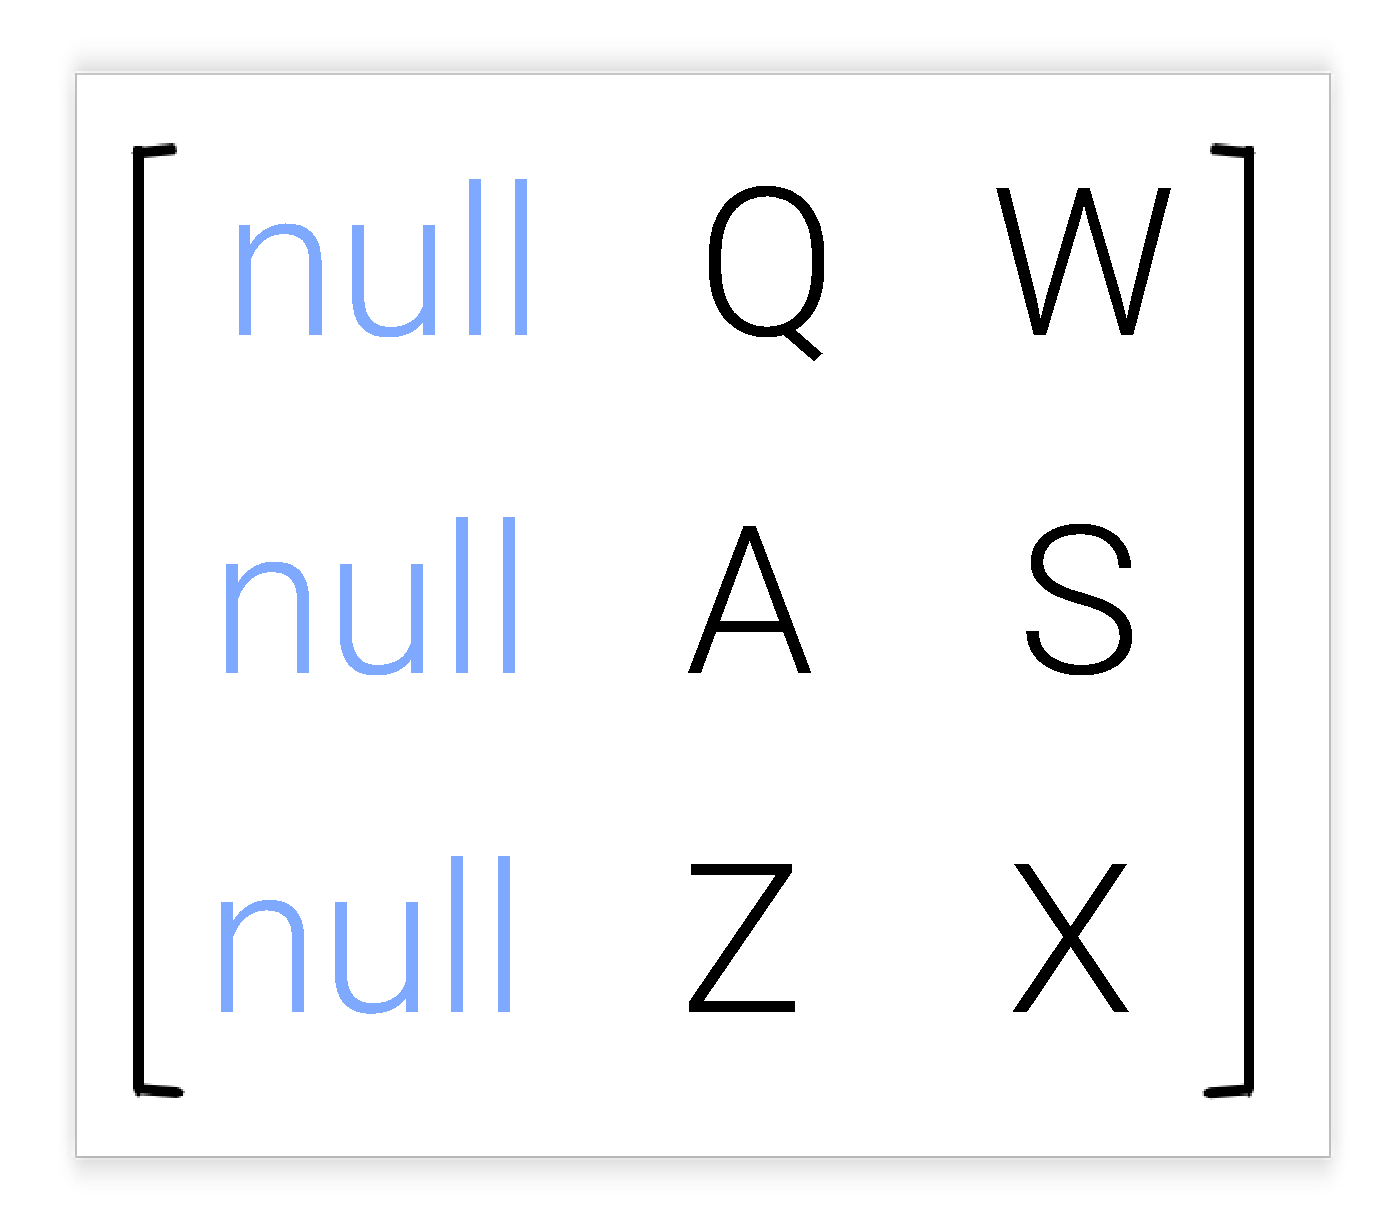
\includegraphics[width=0.5\linewidth,clip=true,trim=0 0 0
% 0]{neighbor_matrix.pdf}
% \caption{Neighbor matrix}
% \label{neighborM}
% \end{minipage}
% \hfill
% \begin{minipage}{.5\textwidth}
% \centering
% 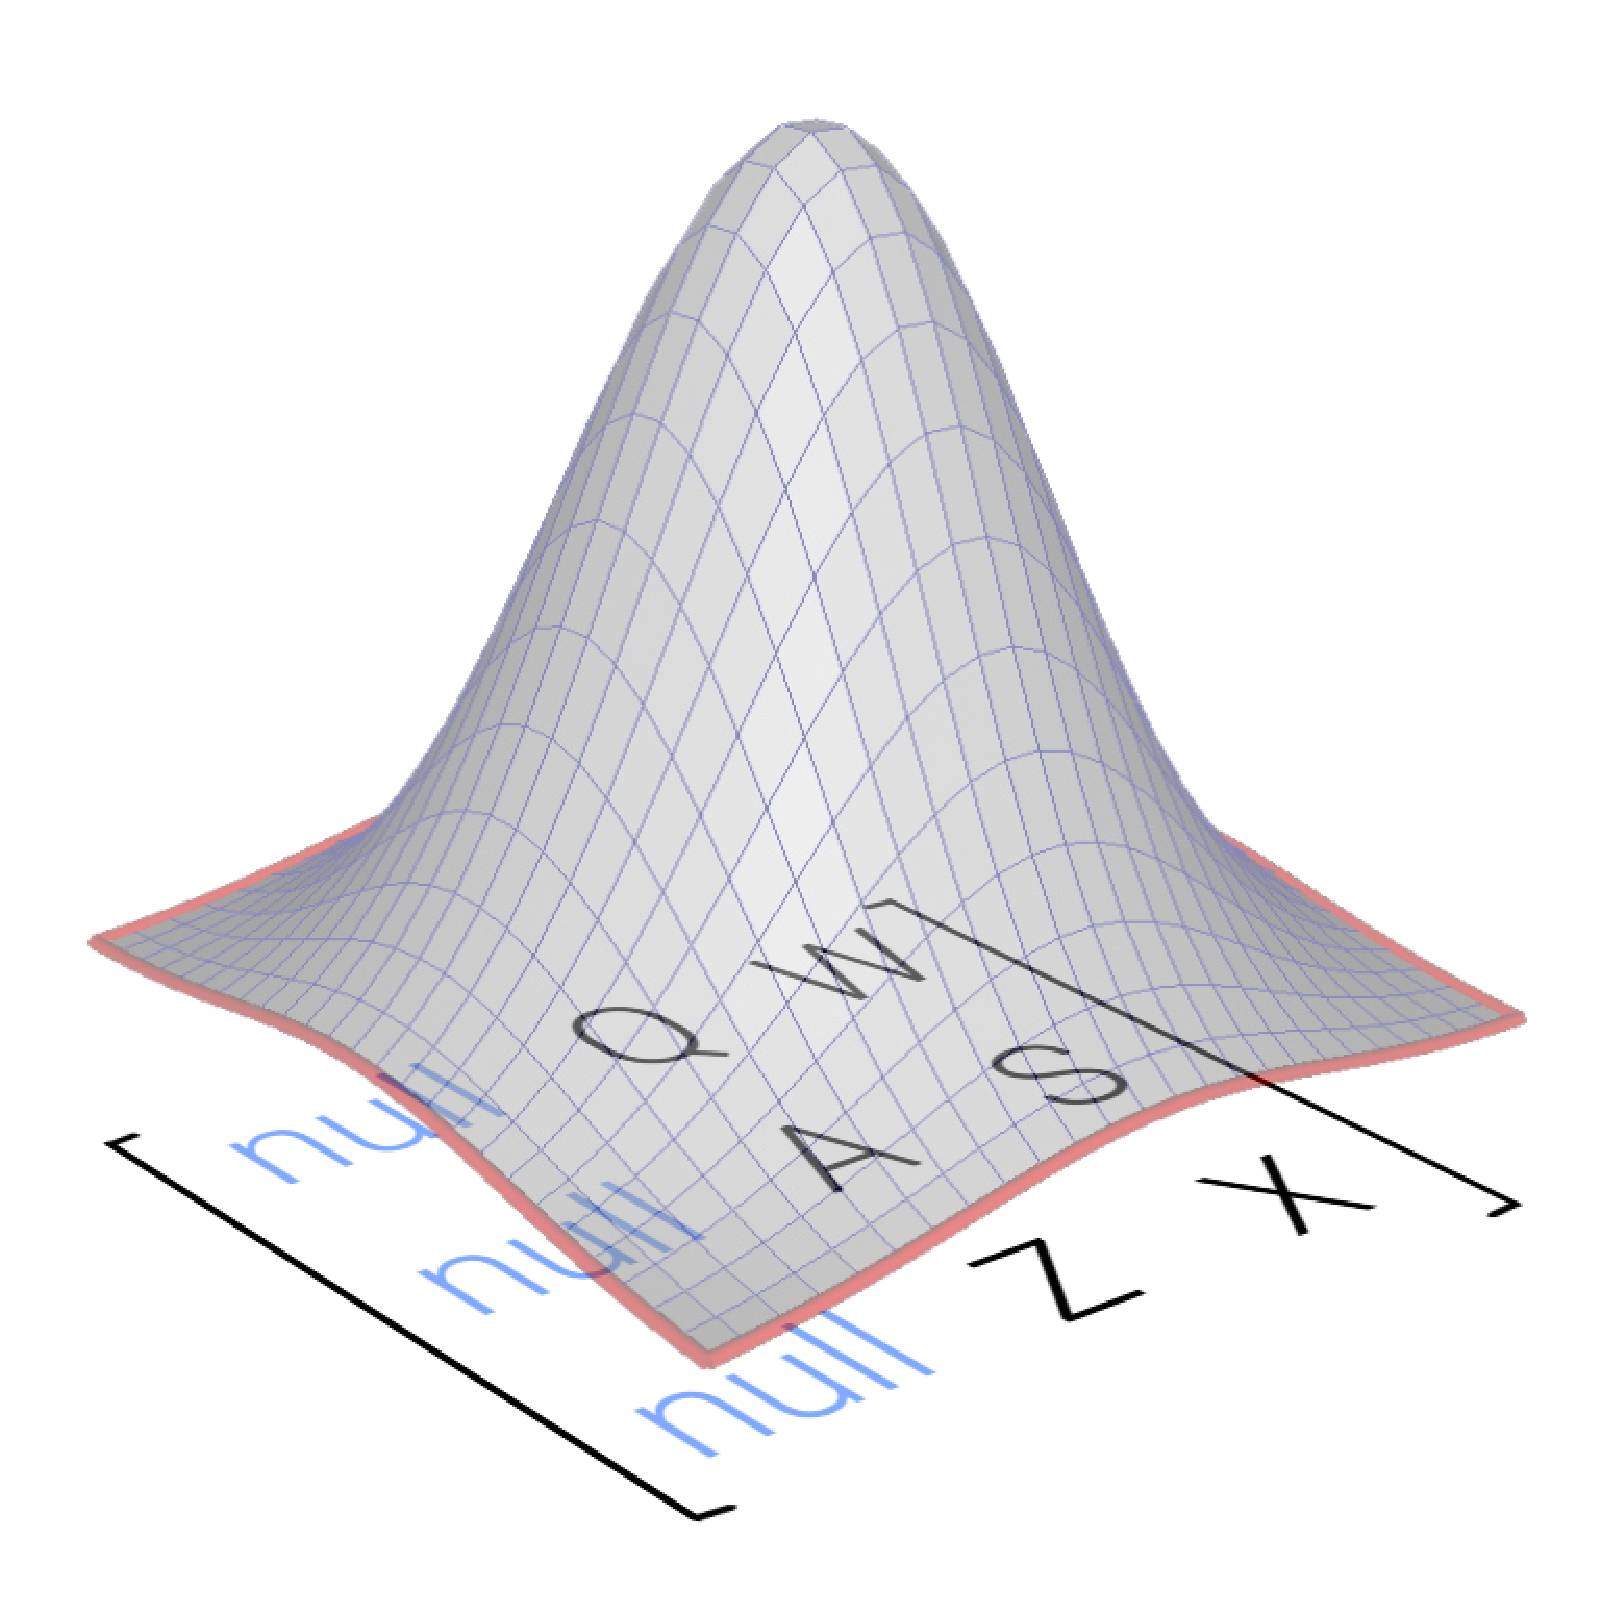
\includegraphics[width=0.5\linewidth,clip=true,trim=0 0 0
% 0]{3D_Gaussian_Perspective.pdf}
% \caption{Gaussian distribution example}
% \label{gaussianD}
% \end{minipage}
% \end{figure}

\begin{figure}[!htbp]
\centering
\subfloat[][Neighbor matrix \label{neighborM}]
{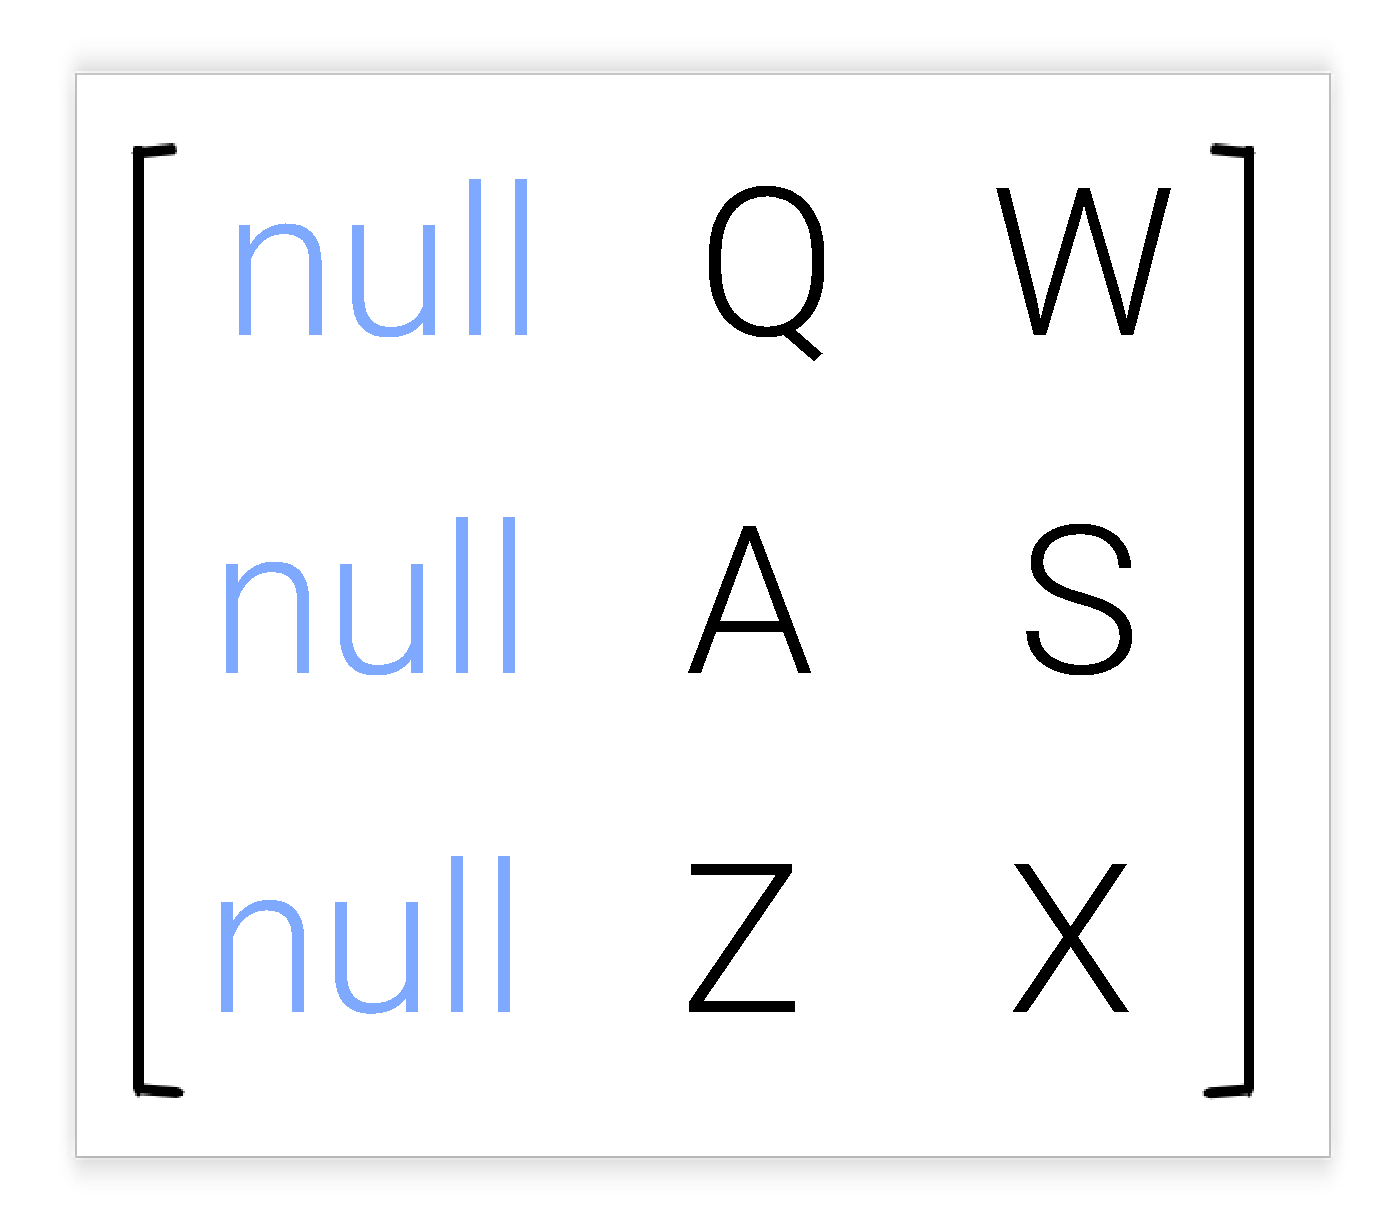
\includegraphics[width=.3\textwidth]{neighbor_matrix.pdf}} \hspace{35pt}
\subfloat[][Gaussian distribution \label{gaussianD}]
{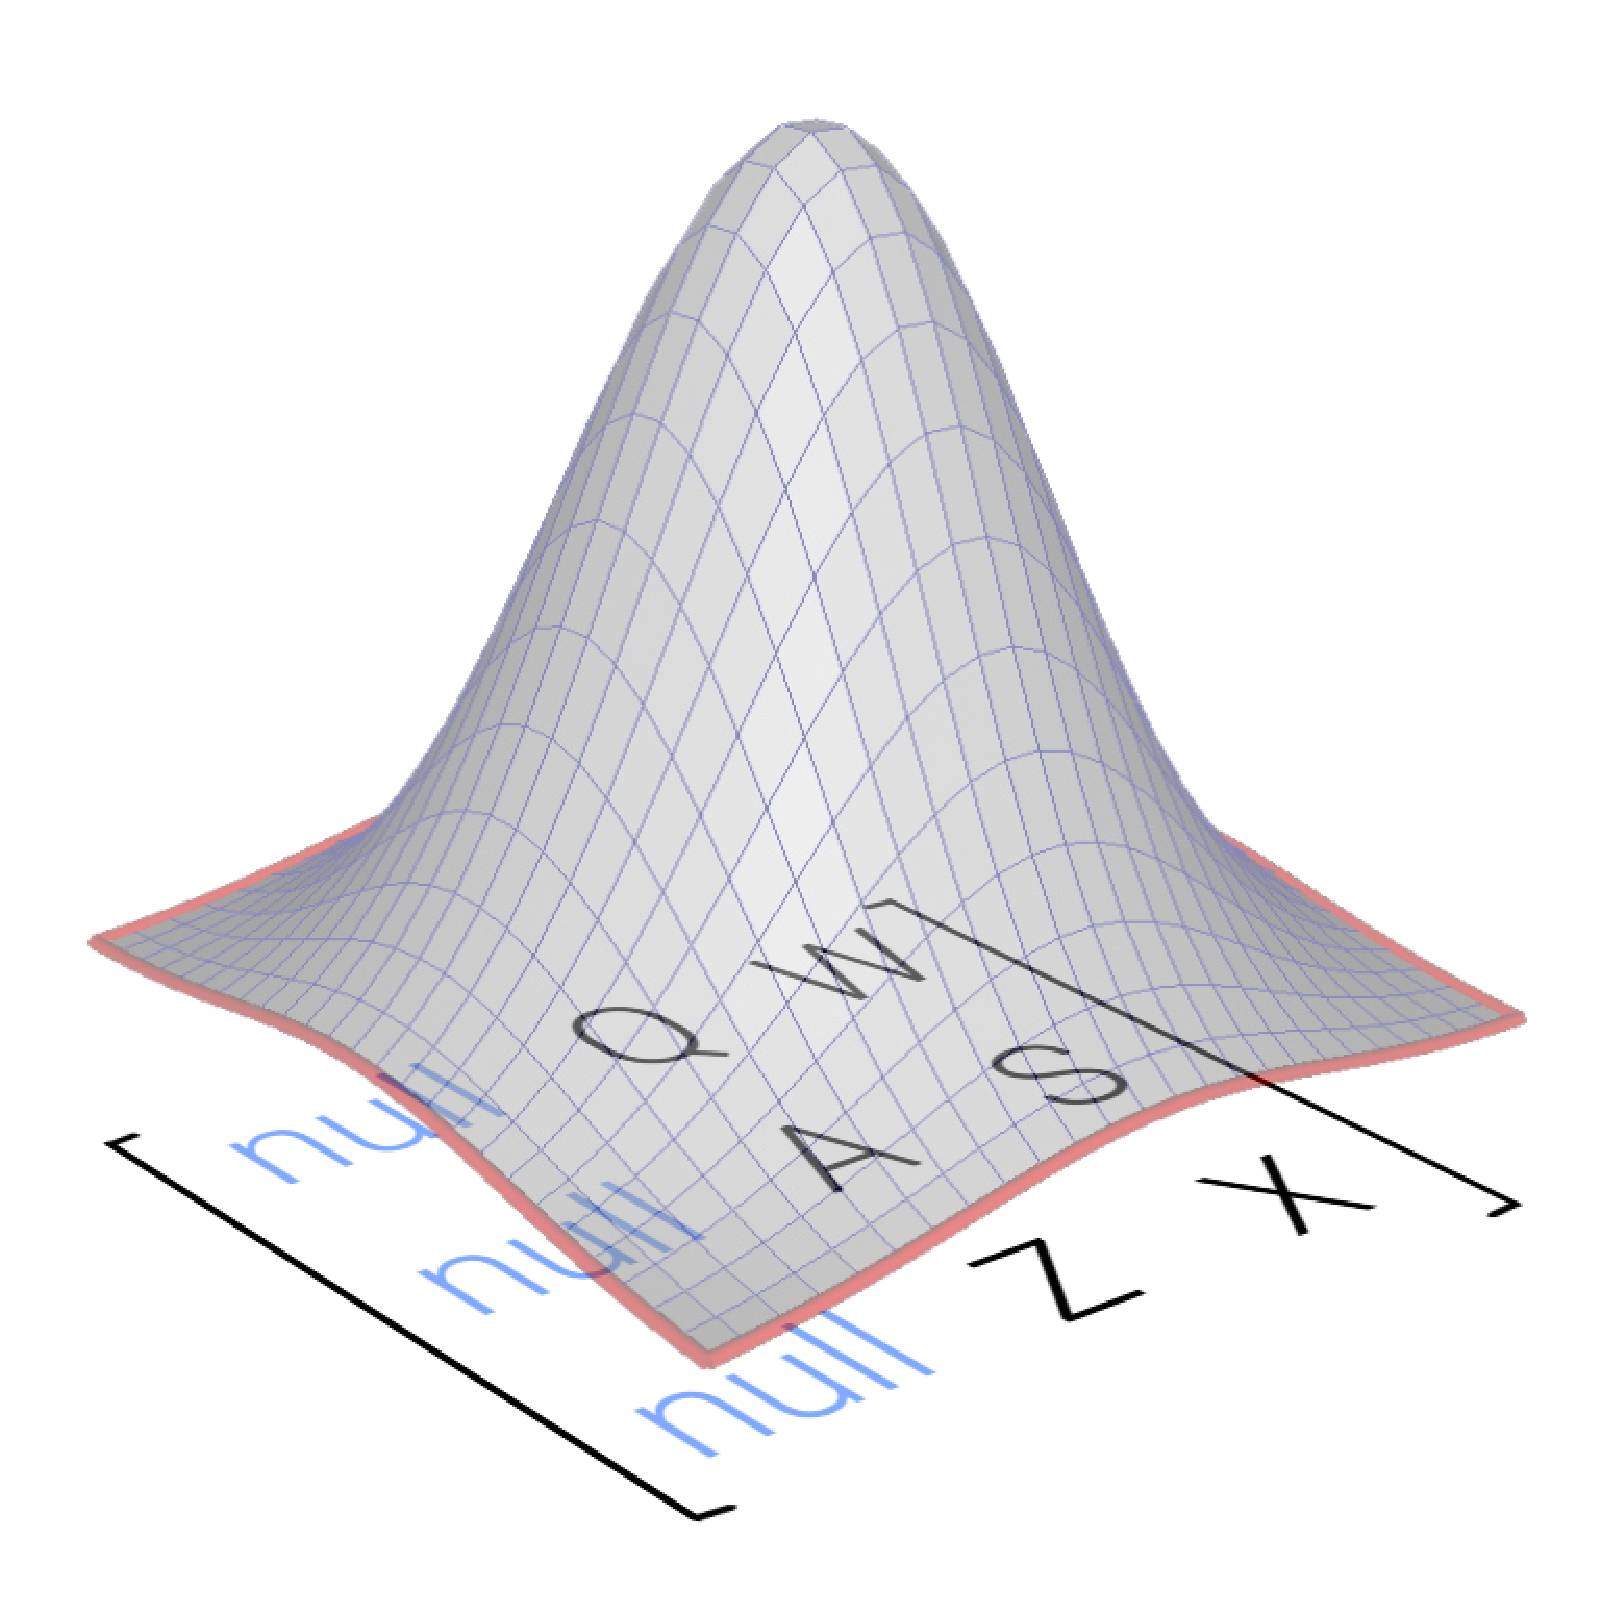
\includegraphics[width=.3\textwidth]{3D_Gaussian_Perspective.pdf}} \\
\caption{Emission distribution example}
\label{matrices}
\end{figure}

\subsection{Training}\label{dataset}
Table~\ref{tab:dataset} reports the datasets used to realize our project: the
data were used to train the model parameters. In
this report we refer to them as \emph{Twitter}~(collection of tweets about apple
and trump), \emph{Swift}~(collection of news, tweets and
blogs text) and \emph{Hybrid}~(Tweet + Swift).

All datasets were previously cleaned from all characters
different from the alphabetical ones(lowercase and uppercase), plus whitespace.
Moreover, urls and mentions were removed from each tweet in order to avoid
noisy samples.

\begin{table}[htbp]
  \centering
  \setlength{\tabcolsep}{0.4em}
  \renewcommand{\arraystretch}{1.2}
    \begin{tabular}{lcr}
    \toprule
    \textbf{Name}  & \textbf{Source} & \textbf{\#characters} \\
    \midrule
    news  & Swift Key  & 204233394 \\
    twitter & Swift Key  & 164456394 \\
    blogs & Swift Key  & 207723793 \\
    apple & Twitter & 2376252 \\
    trump & Twitter & 11849767 \\
    \bottomrule
    $Swift$ & news, twitter, blogs & 576413581 \\
    $Twitter$ & apple, trump & 14226019 \\
    $Hybrid$ & Swift, Twitter & 590639600 \\
    \bottomrule
    \end{tabular}%
    \caption{Dataset information}
  \label{tab:dataset}%
\end{table}%

\subsection{Dictionary}\label{dict}
In order to support and enhance our algorithm, we added a
function which verifies word existence on a dictionary. After the correction of
every word, this function checks whether the corrected word or the original one is included in
the dictionary and returns the matching one, giving priority to the corrected
word in case both are equally present/absent in the dictionary. The dictionary was taken
from NLTK (see \url{www.nltk.org}).

\newpage
\section{Tools and libraries}\label{libraries}
% Table generated by Excel2LaTeX from sheet 'Foglio3'
\begin{table}[!htbp]
  \centering
  \setlength{\tabcolsep}{0.4em}
    \begin{tabularx}{\linewidth}{XlX}
    \toprule
    Library & Source & Description \\
    \midrule
    Hidden-Markov Model &  \url{github.com/Red-devilz/hidden_markov}
    & Python implementation of the hidden markov model \\
    \midrule
    Autowrong & \url{github.com/pwrstudio/autowrong} & Introduces keyboard
    typos into a string \\
    \midrule
    Tweepy & \url{www.tweepy.org} & Python library for accessing the Twitter
    API.
    \\
    \midrule
    Django & \url{www.djangoproject.com} & High-level Python Web
    framework.
    \\
    \bottomrule
    \end{tabularx}%
    \caption{Libraries}
  \label{tab:libraries}%
\end{table}%

% \begin{tabular}{ll}
% Mass of empty crucible & \SI{7.28}{\gram}\\
% Mass of crucible and magnesium before heating & \SI{8.59}{\gram}\\
% Mass of crucible and magnesium oxide after heating & \SI{9.46}{\gram}\\
% Balance used & \#4\\
% Magnesium from sample bottle & \#1
% \end{tabular}

%----------------------------------------------------------------------------------------
%	SECTION 3
%----------------------------------------------------------------------------------------



% \begin{tabular}{ll}
% Mass of magnesium metal & = \SI{8.59}{\gram} - \SI{7.28}{\gram}\\
% & = \SI{1.31}{\gram}\\
% Mass of magnesium oxide & = \SI{9.46}{\gram} - \SI{7.28}{\gram}\\
% & = \SI{2.18}{\gram}\\
% Mass of oxygen & = \SI{2.18}{\gram} - \SI{1.31}{\gram}\\
% & = \SI{0.87}{\gram}
% \end{tabular}
% 
% Because of this reaction, the required ratio is the atomic weight of magnesium: \SI{16.00}{\gram} of oxygen as experimental mass of Mg: experimental mass of oxygen or $\frac{x}{1.31}=\frac{16}{0.87}$ from which, $M_{\ce{Mg}} = 16.00 \times \frac{1.31}{0.87} = 24.1 = \SI{24}{\gram\per\mole}$ (to two significant figures).

%----------------------------------------------------------------------------------------
%	SECTION 4
%----------------------------------------------------------------------------------------

\section{Test and results}\label{analysis}
In the following section we report the results obtained from the test conducted
on our application. First we introduce our test dataset, then we
describe the semantic of our output data, we list our performance metrics and
finally we discuss the results.
Notice that for what concerns the testing we divided the output data depending
on whether the correction was launched having the whole tweet as input or single
words in tweets as input. On the contrary, when evaluating the output data we
only checked if every word of the output text was equals to every word in the ground truth,  types
of correction(on whole tweets/on single words).

\subsection{Data Analysis}\label{dataAnal}


We partitioned the output data by assigning to each word in the analyzed text
three boolean attributes:

\textit{1)} \emph{Perturbed}, which indicates whether the word was
perturbed by Autowrong or not; \textit{2)}
\emph{Corrected}, set to $1$ if the model tried to correct it; \textit{3)}
\emph{True}, set to $1$ if the output word matches the ground truth.
In Figure~\ref{confusionCircle} we reported the representation of how we divided the data.
the circle contains all word which were corrected(\emph{Corrected} = $1$) by our
model.
It is divided in:
\begin{itemize} 
	\item \textbf{corrected-right}: perturbed word which were corrected and match
	the ground truth;
	\item \textbf{corrected-wrong}: word which were corrected badly whether they
	were perturbed or not;
	\item \textbf{not corrected-right}: word not corrected and match the
	ground truth;
	\item \textbf{not corrected-wrong}: missed correction of word.
\end{itemize}

\begin{figure}[hbpt]
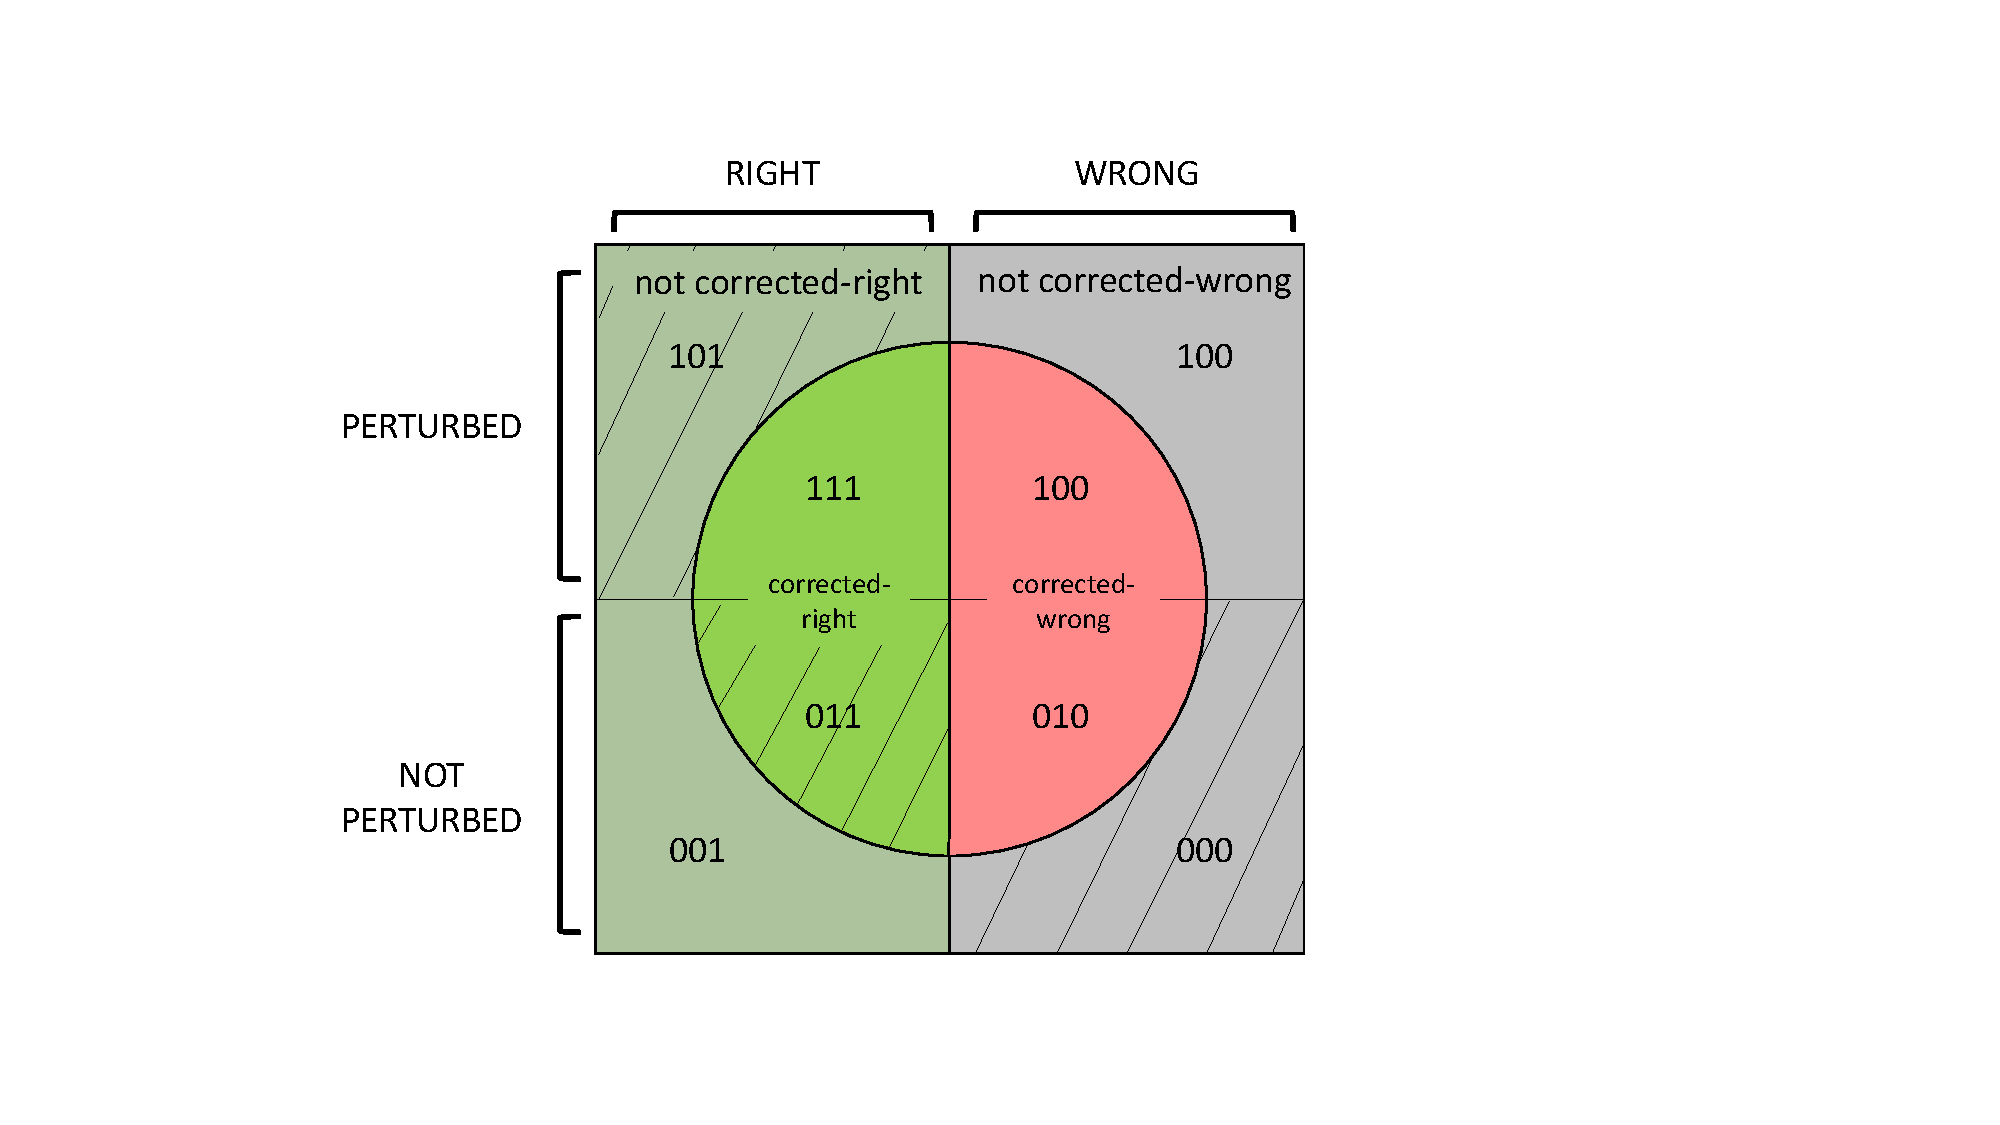
\includegraphics[width=\linewidth,clip=true,trim=100 30 150
60]{confusionCircle.pdf}
\caption{Data representation}
\label{confusionCircle}
\end{figure}

In Table~\ref{tab:features}, all the possible combination of attributes which
define each data set.

% Table generated by Excel2LaTeX from sheet 'Foglio2'
\begin{table}[htbp]
  \centering
    \begin{tabularx}{\linewidth}{ccc|cc}
    %\toprule
    \multicolumn{3}{c}{\textbf{Observation}} &       &  \\
    \midrule
    \textbf{Perturbed} & \textbf{Corrected} & \textbf{True} & \textbf{Description} & \textbf{Evaluation} \\
    \midrule
    0     & 0     & 0     &   -    & impossible \\
    0     & 0     & 1     & not altered observation & correct \\
    0     & 1     & 0     & unnecessary correction & wrong \\
    1     & 0     & 0     & missed correction & wrong \\
    1     & 0     & 1     &   -    & impossible \\
    1     & 1     & 0     & wrong correction & wrong \\
    0     & 1     & 1     &   -    & impossible \\
    1     & 1     & 1     & right  correction & correct \\
    \bottomrule
    \end{tabularx}%
    \caption{Data attributes}
  \label{tab:features}% 
\end{table}%


\subsection{Performance measure}
The combinations of attributes in Table \ref{tab:features} were used to generate
the confusion matrix in Table~\ref{tab:confusionM}. From this matrix we define:
\begin{equation}Precision = \frac{111}{111 + 100}\end{equation}

\begin{equation}Recall = \frac{111}{111 + 010 + 110}\end{equation}

\begin{equation}Accuracy = \frac{111 + 001}{111 + 100 + 010 + 110 +
001}\end{equation}

\begin{equation}F1-measure = 2 * \frac{precision * recall}{precision +
recall}\end{equation}







% Table generated by Excel2LaTeX from sheet 'Foglio5'
% Table generated by Excel2LaTeX from sheet 'Foglio5'
% Table generated by Excel2LaTeX from sheet 'Foglio5'
\begin{table}[htbp]
  \centering
  \setlength{\tabcolsep}{1em}
  \renewcommand{\arraystretch}{1.5}
    \begin{tabular}{cccc}
    \toprule
          &       & \multicolumn{2}{c}{\textbf{Predicted condition}} \\
    \midrule
          &       & T     & F \\
    \multicolumn{1}{c}{\multirow{2}[0]{*}{\textbf{True Condition}}} & T     &
    111(TP) & 100(FN) \\
    \multicolumn{1}{c}{} & F     & {010, 110(FP)} & 001(TN) \\
    \bottomrule \end{tabular}%
    \caption{Confusion matrix}
  \label{tab:confusionM}%
\end{table}%

%
\subsection{Performance evaluation}
The performances were valued on tweets from dataset \emph{Apple} composed by
5700 tweets containing 69 000 words talking about Apple Inc..
\emph{Apple} dataset was previously corrupted with a $5\%$ error
probability thanks to Autowrong, which leads to $25\%$ corrupted words.
The errors simulate the wrong typing of a digit by replacing the intended digit with one of its neighbors.

We ran the Viterbi algorithm with different input values and measured the performance variation. In particular, we experimented different configurations
of Emission Matrix(EM) and Transition Matrix(TM). All experiments were conducted
twice by running the algorithm on the text of the whole tweets first and on
every single word of the tweets then. In the following section we will show the
results in both cases.

Our goal was to establish the best parameter configuration for the analysis and
the model. 
The considered parameters are: 
\begin{itemize}
  \item \emph{Analysis}: defined on \{tweets, words\}, indicates whether the
  analysis was conducted by running the algorithm on the text of the whole
  tweets or on every single word of the tweets;
  \item \emph{Transition Matrix training(TM tr)}: defined on \{\emph{Twitter},
  \emph{Swift}, \emph{Hybrid}\}, indicates the dataset on which the transition
  matrix was trained;
  \item \emph{Emission Matrix distribution(EM distr)}: defined on \{uniform,
  gaussian, custom\}, indicates the distribution of the values in the emission
  matrix;
  \item \emph{EM parameter}: defined on [0.05, 0.95] with a step of $0.05$,
  in case of custom EM distr = custom indicates the probability of pressing the
  intended digit; in case of gaussian EM distr = gaussian indicates the variance value.
\end{itemize}
The possible parameters combination are $2 * 3 * 2 * 19 + 2 * 3 = 234$. In order
to find the best configuration, we first looked for the combination of
``Analysis'', ``TM tr'' and ``EM  distr'' which gives the highest value of
\emph{Accuracy}. For every parameter p, we fixed the remaining two and for every
combination we verified which value of p maximizes the \emph{Accuracy}. In
Table~\ref{tab:tab1}, \ref{tab:tab2} and \ref{tab:tab3}, the best parameter value is called ``Winner''.

From these Tables we assessed that the best combination for the three parameter
is \{$Analysis =$ tweets, $TM tr =$ Hybrid, $EM distr =$ custom\}.
 % Table generated by Excel2LaTeX from sheet 'Sheet1'
\begin{figure}
\centering
 \begin{minipage}{.45\textwidth}
 \centering
   \setlength{\tabcolsep}{0.5em}
    \begin{tabular}{cc|c}
    \toprule
    \multicolumn{2}{c|}{Combination} &  \\
    \textbf{Analysis} & \textbf{TM}    & \textbf{EM Winner} \\
    \midrule
    tweet & Swift & Custom \\
    tweet & Twitter & Custom \\
    tweet & Hybrid & Custom \\
    words & Swift & Custom \\
    words & Twitter & Custom \\
    words & Hybrid & Custom \\
    \bottomrule
    \end{tabular}%
    \captionof{table}{EM best parameter versus Analysis and TM}%
    \label{tab:tab1}%
     

  \setlength{\tabcolsep}{0.5em}
        \begin{tabular}{cc|c}
    \toprule
    \multicolumn{2}{c|}{Combination} &  \\
    \textbf{Analysis} & \textbf{EM}    & \textbf{TM Winner} \\
    \midrule
    tweets & Custom & Hybrid \\
    words & Custom & Hybrid \\
    tweets & Gaussian & Hybrid \\
    words & Gaussian & Hybrid \\
    tweets & Uniform & SwiftKey \\
    words & Uniform & SwiftKey \\
    \bottomrule
        \end{tabular}%
        \captionof{table}{TM best parameter versus Analysis and EM}%
  \label{tab:tab2}%
%\end{table}%
\end{minipage}%
\begin{minipage}{.45\textwidth}
% Table generated by Excel2LaTeX from sheet 'Sheet1'
%\begin{table}[htbp]
  \centering
%   \caption{Add caption}
    \begin{tabular}{cc|c}
    \toprule
    \multicolumn{2}{c|}{Combination} &  \\
    \textbf{EM} & \textbf{TM} & \textbf{Analysis Winner} \\
    \midrule
    Swift & Custom & tweets \\
    Swift & Gaussian & tweets \\
    Swift & Uniform & tweets \\
    Hybrid & Custom & tweets \\
    Hybrid & Gaussian & tweets \\
    Hybrid & Uniform & tweets \\
    Twitter & Custom & tweets \\
    Twitter & Gaussian & tweets \\
    Twitter & Uniform & tweets \\
    \bottomrule
    \end{tabular}%
    \captionof{table}{Analysis best parameter versus EM and TM}
  \label{tab:tab3}%
%\end{table}%
\end{minipage}%
\end{figure}%
%%Emission matrix


For what concerns the gaussian/custom distribution of emissions, we tested them
with different \emph{EM parameters} in order to understand
how the performances change.
% %Gaussian
In Figure~\ref{gaussG} we resume the results obtained with
different variance settings  word analysis and tweet analysis. The
performance valued was the number of words in each output data set(see
Section~\ref{dataAnal}).

\begin{figure}[!htbp]
\centering
\subfloat[][Analysis: tweets - TM training set: Hybrid \label{gaussTweet}]
{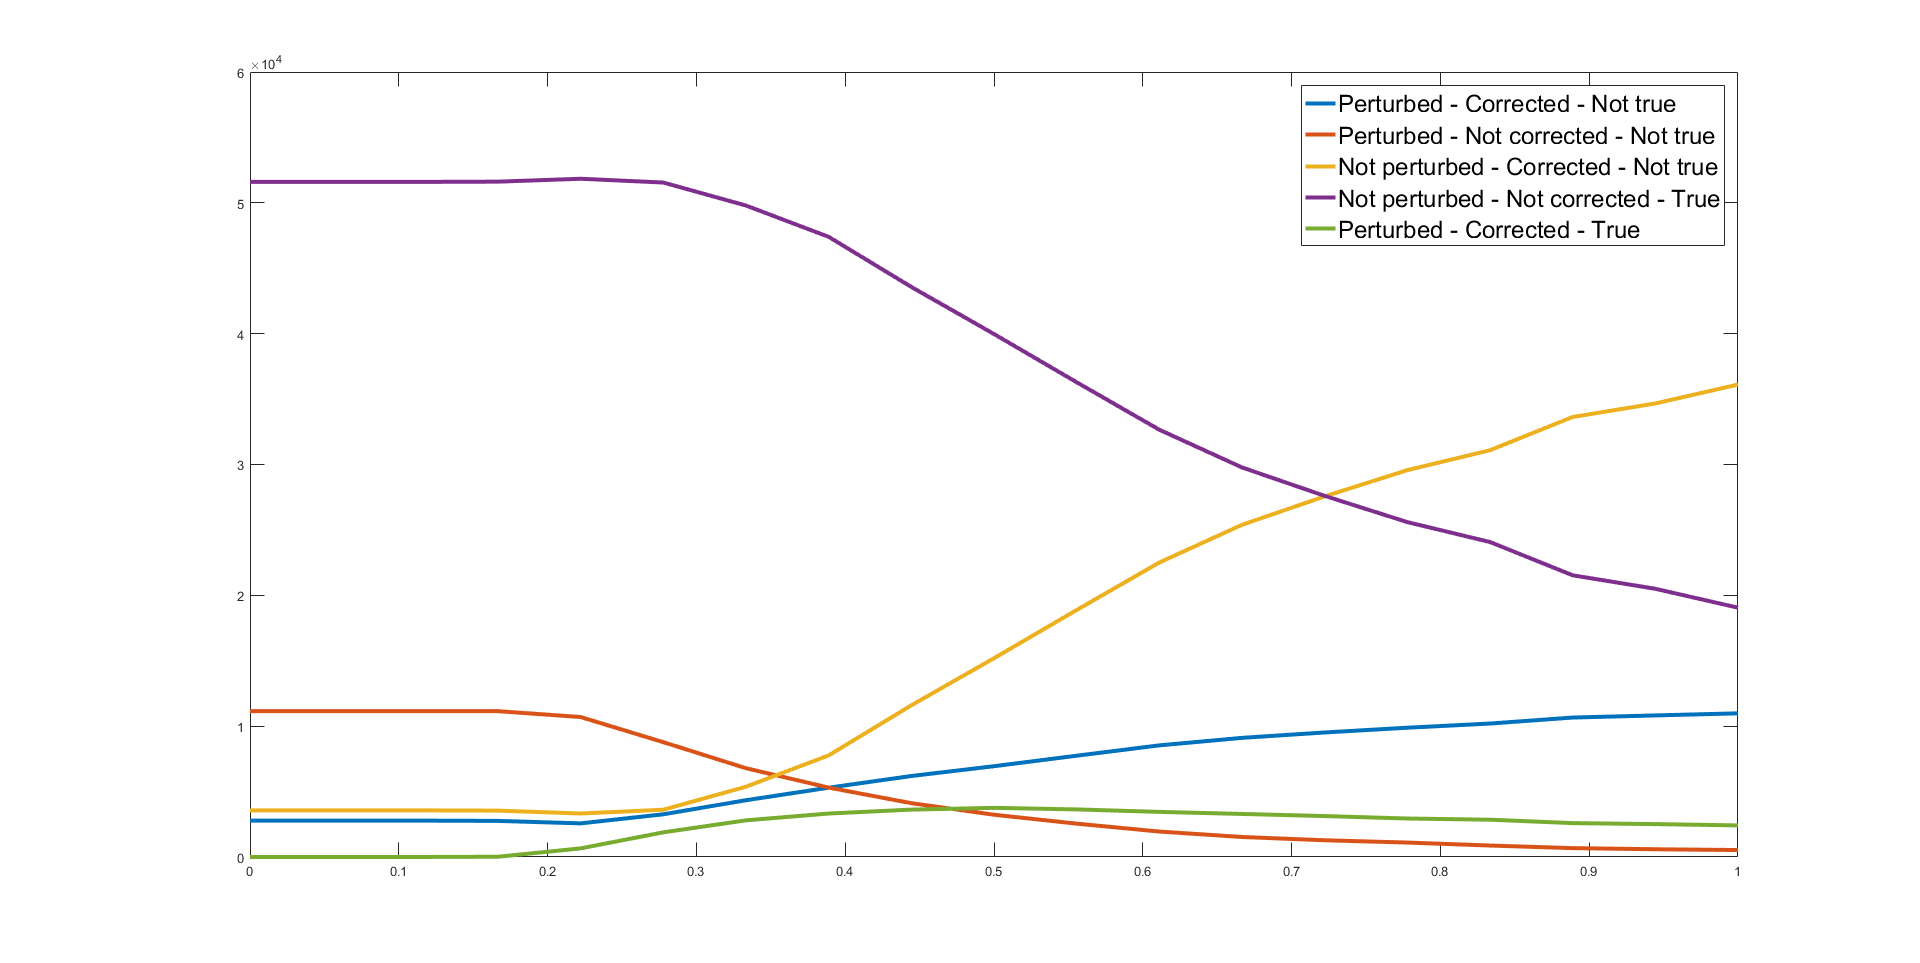
\includegraphics[width=1\textwidth]{tweets_hybrid_gaussian.png}} \hspace{35pt}
\subfloat[][Analysis: words - TM training set: Hybrid \label{gaussWord}]
{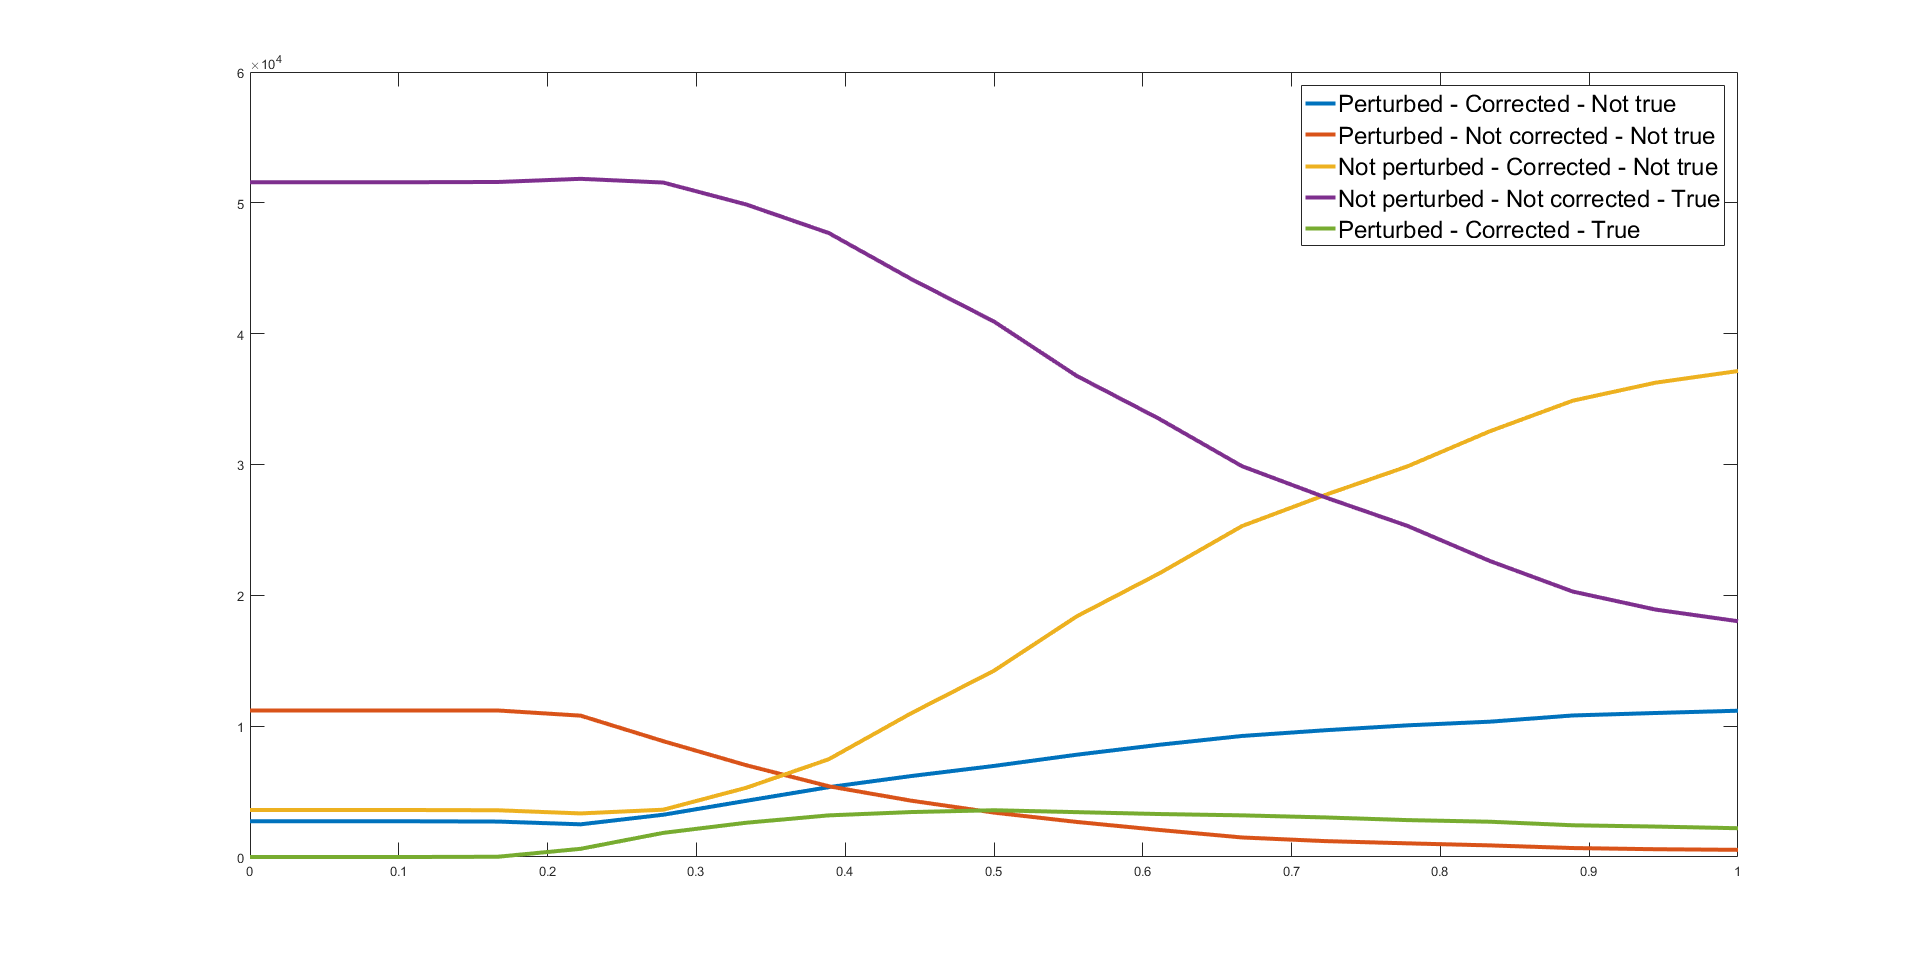
\includegraphics[width=1\textwidth]{words_hybrid_gaussian.png}} \\
\caption{Gaussian distribution - variance influence on output data}
\label{gaussG}
\end{figure}

%Custom
Figure~\ref{customG} shows how the probability of pressing the intended digit
affects the performance word analysis and tweet analysis. The
performance valued was the number of words in each output data set(see
Section~\ref{dataAnal}).

\begin{figure}[!htbp]
\centering
\subfloat[][Analysis: tweets - TM training set: Hybrid \label{customTweet}]
{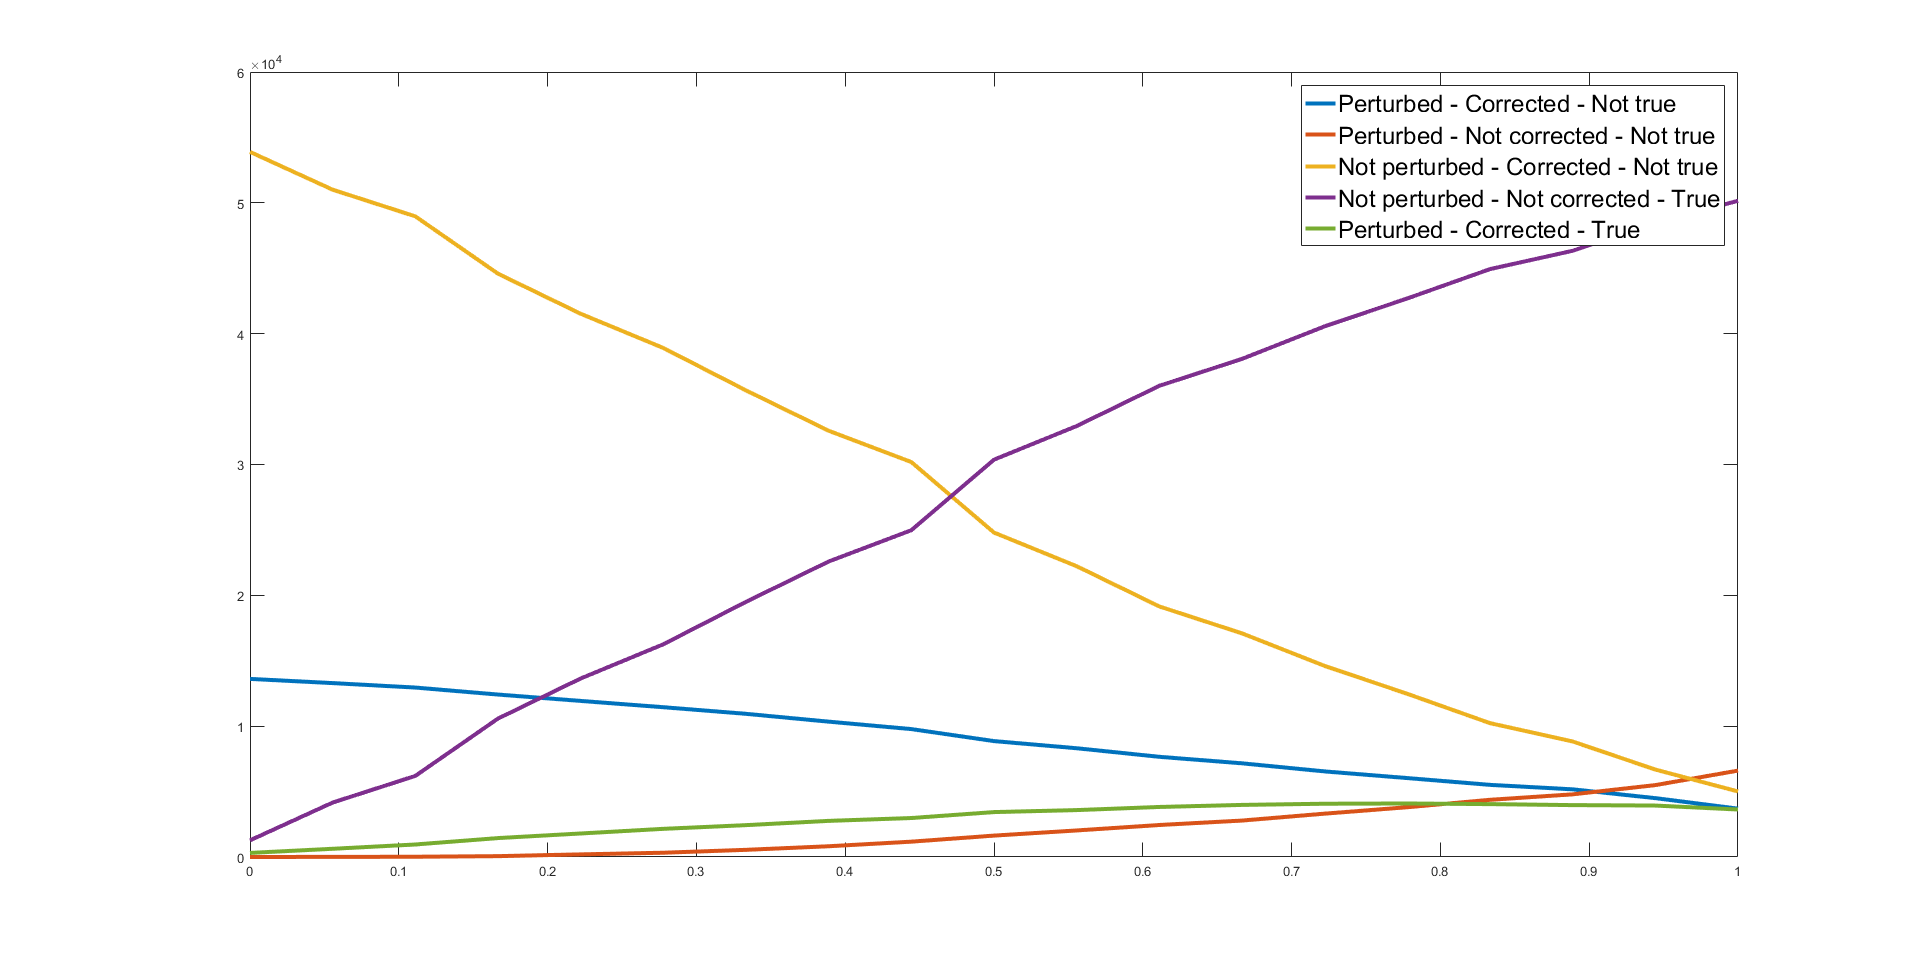
\includegraphics[width=1\textwidth]{tweets_hybrid_custom.png}} \hspace{35pt}
\subfloat[][Analysis: words - TM training set: Hybrid \label{customWord}]
{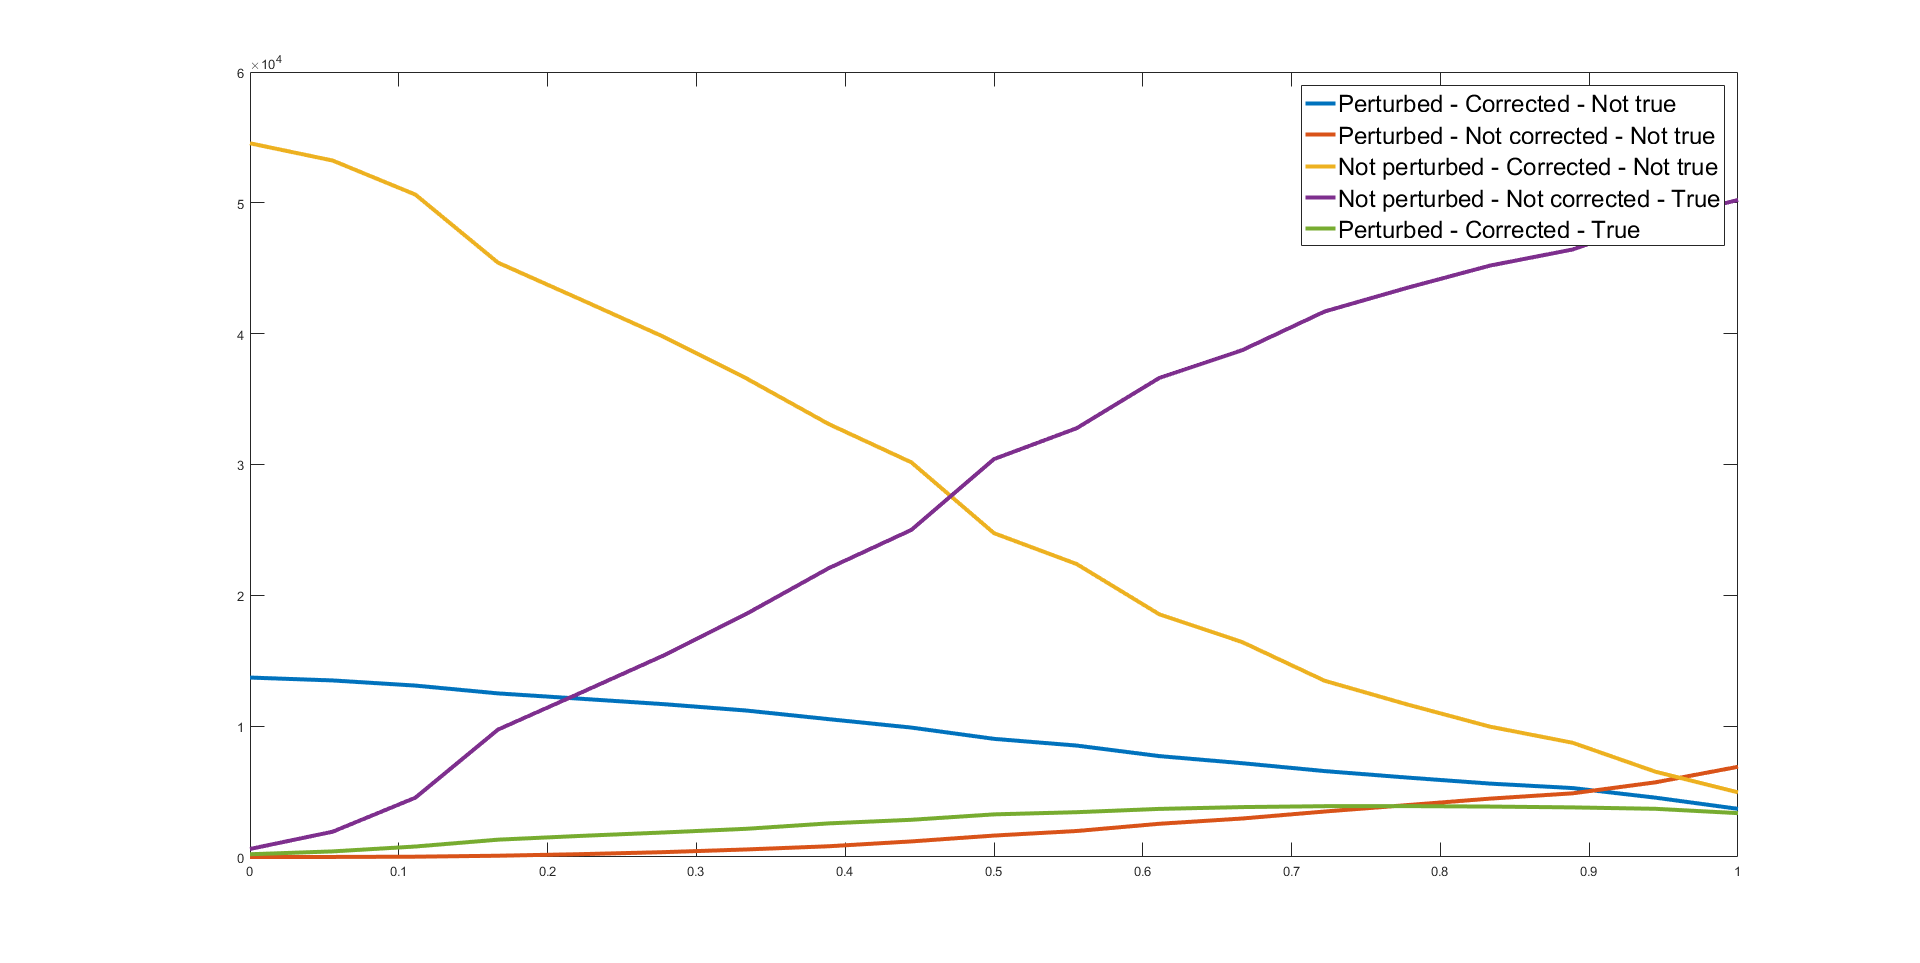
\includegraphics[width=1\textwidth]{words_hybrid_custom.png}} \\
\caption{Custom distribution - intended digit probability influence on
output data}
\label{customG}
\end{figure}

After our experiments we established that the best value for the parameter is
$EM parameter =$ 0.35, in case of \emph{EM distr} = gaussian; $EM parameter =$
0.95, in case of \emph{EM distr} = custom.

In Table~\ref{tab:bestResults}, the best results obtained with the best
parameters configuration.

%frequency table
% Table generated by Excel2LaTeX from sheet 'Foglio7'
% Table generated by Excel2LaTeX from sheet 'Foglio10'
\begin{table}[htbp]
  \centering
    \begin{tabular}{cccccccc}
    \toprule
    \textbf{Analysis} & \textbf{TM tr} & \textbf{EM distr} & \textbf{EM p} & \textbf{Prec} & \textbf{Rec} & \textbf{F1} & \textbf{Acc} \\
    \midrule
    tweets & Hybrid & custom & 0.95  & 0.2942 & 0.3547 & 0.3216 & 0.7784 \\
    \bottomrule
    \end{tabular}%
  \caption{Best results on dataset apple}
\end{table}%
\label{tab:bestResults}%

The test presented was conducted without the support of our dictionary(see
Section~\ref{dict}). After its introduction, we observed a linear increase of
the performance metrics. Table~\ref{tab:final} shows a sample of the final
results that we obtained from testing dataset \emph{Apple}.

% Table generated by Excel2LaTeX from sheet 'Foglio8'
\begin{table}[htbp]
  \centering
    \begin{tabular}{rlllllllll}
    \toprule
    \textbf{Rank} & \textbf{Analysis} & \textbf{Dict} & \textbf{TM tr} & \textbf{EM distr} & \textbf{EM p} & \textbf{Prec} & \textbf{Rec} & \textbf{F1} & \textbf{Acc} \\
    \midrule
    1     & tweets & NLTK  & Twitter & custom & 0.95  & 0.3364 & 0.3688 & 0.3519
    & 0.8006 \\
    2     & tweets & NLTK  & Swift & custom & 0.95  & 0.3303 & 0.3432 & 0.3366 &
    0.7991 \\
    5     & tweets & NLTK  & Twitter & gaussian & 0.35 & 0.2761 & 0.3107 &
    0.2924 & 0.7900\\
    19    & tweets & \multicolumn{1}{c}{-} & Hybrid & custom & 0.95  & 0.2942 &
    0.3547 & 0.3216 & 0.7784 \\
    23    & words & \multicolumn{1}{c}{-} & Hybrid & custom & 0.95  & 0.2799 &
    0.3272 & 0.3017 & 0.7754 \\
    24    & words & NLTK  & Twitter & gaussian & 0.35  & 0.2480 & 0.2981 &
    0.2708 & 0.7754 \\
    30    & words & NLTK  & Hybrid & gaussian & 0.3   & 0.2110 & 0.1684 & 0.1873
    & 0.7736 \\
    31    & tweets & \multicolumn{1}{c}{-} & Hybrid & gaussian & 0.3   & 0.2152
    & 0.1769 & 0.1942 & 0.7734 \\
    339   & tweets & NLTK  & Swift & uniform & \multicolumn{1}{c}{-} & 0.0326 &
    0.6054 & 0.0619 & 0.4814 \\
    632   & tweets & \multicolumn{1}{c}{-} & Swift & uniform &
    \multicolumn{1}{c}{-} & 0.0227 & 0.9559 & 0.0444 & 0.1625 \\
    \bottomrule
    \end{tabular}%
    \caption{Final results on Apple dataset}
  \label{tab:final}%
\end{table}%

\subsection{Word prediction analysis}
In this section we show some examples of how our model corrects or nor frequent
and infrequent words.

The most frequent word is ``Apple''. This word is perturbed in different ways:
some of them are corrected by our model, some remain corrupted. For instance,
``Apole'', ``Appoe'' and ``Alple'' are all samples of uncorrected perturbation.
In this case, even if the probability of 'pl' Is higher that 'po' and 'pp', the
sequence probability is higher for 'Appp' and 'Apol' than 'Appl', hence our
model doesn't correct the words.
On the other hand, the model succeds in the correction when the word is
perturbed as ``Aople'', ``Apple" or ``Wpple'': in these cases the error is
not exploting the model weaknesses.

Another example of common wrongly corrected word is ``you'', perturbed as
``yoh'' or  ``yoj''. Our model corrects it as ``yon'' because the emission
probability of the 'n' and 'u' are equal, but the transition probability is
higher for bigram 'o-n' than 'o-u'.

The last example regards an uncommon word which is not corrected when perturbed.
``Liveroooo'', perturbation of ``Liverpool'', is not corrected because the
bigram 'oo' is a common one, and our system is unable to handle errors of triple
or more letters repeated.

\section{HMMispelling demo}
%insert screenshot
As result of our project, we introduce our demo ``HMMispelling''. The demo
offers a Graphic User Interface and two modes: an interactive mode where the
user can type his message and check the real time correction and an automatic
one which shows the real time correction of a stream of real tweets.

The pipeline of our application is divided in ..steps:
\begin{itemize}
  \item Takes the input text
  \item Infers the correction of the eventual typos from the model
  \item returns the corrected text
\end{itemize}

\section{Conclusions}
In our project we developed an application able to correct keyboard typos thanks
to the use of an Hidden Markov Model.  We trained the model parameters and
tested the possible parameters combinations in order to find the best
configuration for the model. Moreover, we added a dictionary to support the
correction task. Finally we analyzed the results. We don't have high
performances due to our model weakness: the fact that it is based on bigram
frequencies and not on the whole word probability often leads the Viterbi
algorithm to accept perturbed words; if all the bigrams in a word have high
probability to occur, the model can't establish if it is a perturbed or a
corrected word. Future enhancements could be to use a Markov Chain and replace
the bigram frequencies with longer engrams.

% The atomic weight of magnesium is concluded to be \SI{24}{\gram\per\mol}, as determined by the stoichiometry of its chemical combination with oxygen. This result is in agreement with the accepted value.
% 
% \begin{figure}[h]
% \begin{center}
% %%\includegraphics[width=0.65\textwidth]{placeholder} % Include the image
% % placeholder.png
% \caption{Figure caption.}
% \end{center}
% \end{figure}
% 
% %----------------------------------------------------------------------------------------
% %	SECTION 5
% %----------------------------------------------------------------------------------------
% 
% \section{Discussion of Experimental Uncertainty}
% 
% The accepted value (periodic table) is \SI{24.3}{\gram\per\mole} \cite{Smith:2012qr}. The percentage discrepancy between the accepted value and the result obtained here is 1.3\%. Because only a single measurement was made, it is not possible to calculate an estimated standard deviation.
% 
% The most obvious source of experimental uncertainty is the limited precision of the balance. Other potential sources of experimental uncertainty are: the reaction might not be complete; if not enough time was allowed for total oxidation, less than complete oxidation of the magnesium might have, in part, reacted with nitrogen in the air (incorrect reaction); the magnesium oxide might have absorbed water from the air, and thus weigh ``too much." Because the result obtained is close to the accepted value it is possible that some of these experimental uncertainties have fortuitously cancelled one another.
% 
% %----------------------------------------------------------------------------------------
% %	SECTION 6
% %----------------------------------------------------------------------------------------
% 
% \section{Answers to Definitions}
% 
% \begin{enumerate}
% \begin{item}
% The \emph{atomic weight of an element} is the relative weight of one of its atoms compared to C-12 with a weight of 12.0000000$\ldots$, hydrogen with a weight of 1.008, to oxygen with a weight of 16.00. Atomic weight is also the average weight of all the atoms of that element as they occur in nature.
% \end{item}
% \begin{item}
% The \emph{units of atomic weight} are two-fold, with an identical numerical value. They are g/mole of atoms (or just g/mol) or amu/atom.
% \end{item}
% \begin{item}
% \emph{Percentage discrepancy} between an accepted (literature) value and an experimental value is
% \begin{equation*}
% \frac{\mathrm{experimental\;result} - \mathrm{accepted\;result}}{\mathrm{accepted\;result}}
% \end{equation*}
% \end{item}
% \end{enumerate}

%----------------------------------------------------------------------------------------
%	BIBLIOGRAPHY
%----------------------------------------------------------------------------------------

\bibliographystyle{apalike}

\bibliography{sample}

%----------------------------------------------------------------------------------------


\end{document}
